
%% bare_conf.tex
%% V1.4b
%% 2015/08/26
%% by Michael Shell
%% See:
%% http://www.michaelshell.org/
%% for current contact information.
%%
%% This is a skeleton file demonstrating the use of IEEEtran.cls
%% (requires IEEEtran.cls version 1.8b or later) with an IEEE
%% conference paper.
%%
%% Support sites:
%% http://www.michaelshell.org/tex/ieeetran/
%% http://www.ctan.org/pkg/ieeetran
%% and
%% http://www.ieee.org/

%%*************************************************************************
%% Legal Notice:
%% This code is offered as-is without any warranty either expressed or
%% implied; without even the implied warranty of MERCHANTABILITY or
%% FITNESS FOR A PARTICULAR PURPOSE! 
%% User assumes all risk.
%% In no event shall the IEEE or any contributor to this code be liable for
%% any damages or losses, including, but not limited to, incidental,
%% consequential, or any other damages, resulting from the use or misuse
%% of any information contained here.
%%
%% All comments are the opinions of their respective authors and are not
%% necessarily endorsed by the IEEE.
%%
%% This work is distributed under the LaTeX Project Public License (LPPL)
%% ( http://www.latex-project.org/ ) version 1.3, and may be freely used,
%% distributed and modified. A copy of the LPPL, version 1.3, is included
%% in the base LaTeX documentation of all distributions of LaTeX released
%% 2003/12/01 or later.
%% Retain all contribution notices and credits.
%% ** Modified files should be clearly indicated as such, including  **
%% ** renaming them and changing author support contact information. **
%%*************************************************************************


% *** Authors should verify (and, if needed, correct) their LaTeX system  ***
% *** with the testflow diagnostic prior to trusting their LaTeX platform ***
% *** with production work. The IEEE's font choices and paper sizes can   ***
% *** trigger bugs that do not appear when using other class files.       ***                          ***
% The testflow support page is at:
% http://www.michaelshell.org/tex/testflow/



\documentclass[conference]{IEEEtran}
% Some Computer Society conferences also require the compsoc mode option,
% but others use the standard conference format.
%
% If IEEEtran.cls has not been installed into the LaTeX system files,
% manually specify the path to it like:
% \documentclass[conference]{../sty/IEEEtran}





% Some very useful LaTeX packages include:
% (uncomment the ones you want to load)


% *** MISC UTILITY PACKAGES ***
%
%\usepackage{ifpdf}
% Heiko Oberdiek's ifpdf.sty is very useful if you need conditional
% compilation based on whether the output is pdf or dvi.
% usage:
% \ifpdf
%   % pdf code
% \else
%   % dvi code
% \fi
% The latest version of ifpdf.sty can be obtained from:
% http://www.ctan.org/pkg/ifpdf
% Also, note that IEEEtran.cls V1.7 and later provides a builtin
% \ifCLASSINFOpdf conditional that works the same way.
% When switching from latex to pdflatex and vice-versa, the compiler may
% have to be run twice to clear warning/error messages.






% *** CITATION PACKAGES ***
%
\usepackage{cite}
% cite.sty was written by Donald Arseneau
% V1.6 and later of IEEEtran pre-defines the format of the cite.sty package
% \cite{} output to follow that of the IEEE. Loading the cite package will
% result in citation numbers being automatically sorted and properly
% "compressed/ranged". e.g., [1], [9], [2], [7], [5], [6] without using
% cite.sty will become [1], [2], [5]--[7], [9] using cite.sty. cite.sty's
% \cite will automatically add leading space, if needed. Use cite.sty's
% noadjust option (cite.sty V3.8 and later) if you want to turn this off
% such as if a citation ever needs to be enclosed in parenthesis.
% cite.sty is already installed on most LaTeX systems. Be sure and use
% version 5.0 (2009-03-20) and later if using hyperref.sty.
% The latest version can be obtained at:
% http://www.ctan.org/pkg/cite
% The documentation is contained in the cite.sty file itself.






% *** GRAPHICS RELATED PACKAGES ***
%
\ifCLASSINFOpdf
   \usepackage[pdftex]{graphicx}
  % declare the path(s) where your graphic files are
   \graphicspath{ {images/} }
  % and their extensions so you won't have to specify these with
  % every instance of \includegraphics
   \DeclareGraphicsExtensions{.pdf,.jpeg,.png}
\else
  % or other class option (dvipsone, dvipdf, if not using dvips). graphicx
  % will default to the driver specified in the system graphics.cfg if no
  % driver is specified.
  % \usepackage[dvips]{graphicx}
  % declare the path(s) where your graphic files are
  % \graphicspath{{../eps/}}
  % and their extensions so you won't have to specify these with
  % every instance of \includegraphics
  % \DeclareGraphicsExtensions{.eps}
\fi
% graphicx was written by David Carlisle and Sebastian Rahtz. It is
% required if you want graphics, photos, etc. graphicx.sty is already
% installed on most LaTeX systems. The latest version and documentation
% can be obtained at: 
% http://www.ctan.org/pkg/graphicx
% Another good source of documentation is "Using Imported Graphics in
% LaTeX2e" by Keith Reckdahl which can be found at:
% http://www.ctan.org/pkg/epslatex
%
% latex, and pdflatex in dvi mode, support graphics in encapsulated
% postscript (.eps) format. pdflatex in pdf mode supports graphics
% in .pdf, .jpeg, .png and .mps (metapost) formats. Users should ensure
% that all non-photo figures use a vector format (.eps, .pdf, .mps) and
% not a bitmapped formats (.jpeg, .png). The IEEE frowns on bitmapped formats
% which can result in "jaggedy"/blurry rendering of lines and letters as
% well as large increases in file sizes.
%
% You can find documentation about the pdfTeX application at:
% http://www.tug.org/applications/pdftex





% *** MATH PACKAGES ***
%
\usepackage{amsmath}
% A popular package from the American Mathematical Society that provides
% many useful and powerful commands for dealing with mathematics.
%
% Note that the amsmath package sets \interdisplaylinepenalty to 10000
% thus preventing page breaks from occurring within multiline equations. Use:
%\interdisplaylinepenalty=2500
% after loading amsmath to restore such page breaks as IEEEtran.cls normally
% does. amsmath.sty is already installed on most LaTeX systems. The latest
% version and documentation can be obtained at:
% http://www.ctan.org/pkg/amsmath





% *** SPECIALIZED LIST PACKAGES ***
%
\usepackage{algorithmic}
% algorithmic.sty was written by Peter Williams and Rogerio Brito.
% This package provides an algorithmic environment fo describing algorithms.
% You can use the algorithmic environment in-text or within a figure
% environment to provide for a floating algorithm. Do NOT use the algorithm
% floating environment provided by algorithm.sty (by the same authors) or
% algorithm2e.sty (by Christophe Fiorio) as the IEEE does not use dedicated
% algorithm float types and packages that provide these will not provide
% correct IEEE style captions. The latest version and documentation of
% algorithmic.sty can be obtained at:
% http://www.ctan.org/pkg/algorithms
% Also of interest may be the (relatively newer and more customizable)
% algorithmicx.sty package by Szasz Janos:
% http://www.ctan.org/pkg/algorithmicx




% *** ALIGNMENT PACKAGES ***
%
\usepackage{array}
% Frank Mittelbach's and David Carlisle's array.sty patches and improves
% the standard LaTeX2e array and tabular environments to provide better
% appearance and additional user controls. As the default LaTeX2e table
% generation code is lacking to the point of almost being broken with
% respect to the quality of the end results, all users are strongly
% advised to use an enhanced (at the very least that provided by array.sty)
% set of table tools. array.sty is already installed on most systems. The
% latest version and documentation can be obtained at:
% http://www.ctan.org/pkg/array


% IEEEtran contains the IEEEeqnarray family of commands that can be used to
% generate multiline equations as well as matrices, tables, etc., of high
% quality.




% *** SUBFIGURE PACKAGES ***
%\ifCLASSOPTIONcompsoc
%  \usepackage[caption=false,font=normalsize,labelfont=sf,textfont=sf]{subfig}
%\else
%  \usepackage[caption=false,font=footnotesize]{subfig}
%\fi
% subfig.sty, written by Steven Douglas Cochran, is the modern replacement
% for subfigure.sty, the latter of which is no longer maintained and is
% incompatible with some LaTeX packages including fixltx2e. However,
% subfig.sty requires and automatically loads Axel Sommerfeldt's caption.sty
% which will override IEEEtran.cls' handling of captions and this will result
% in non-IEEE style figure/table captions. To prevent this problem, be sure
% and invoke subfig.sty's "caption=false" package option (available since
% subfig.sty version 1.3, 2005/06/28) as this is will preserve IEEEtran.cls
% handling of captions.
% Note that the Computer Society format requires a larger sans serif font
% than the serif footnote size font used in traditional IEEE formatting
% and thus the need to invoke different subfig.sty package options depending
% on whether compsoc mode has been enabled.
%
% The latest version and documentation of subfig.sty can be obtained at:
% http://www.ctan.org/pkg/subfig




% *** FLOAT PACKAGES ***
%
\usepackage{fixltx2e}
% fixltx2e, the successor to the earlier fix2col.sty, was written by
% Frank Mittelbach and David Carlisle. This package corrects a few problems
% in the LaTeX2e kernel, the most notable of which is that in current
% LaTeX2e releases, the ordering of single and double column floats is not
% guaranteed to be preserved. Thus, an unpatched LaTeX2e can allow a
% single column figure to be placed prior to an earlier double column
% figure.
% Be aware that LaTeX2e kernels dated 2015 and later have fixltx2e.sty's
% corrections already built into the system in which case a warning will
% be issued if an attempt is made to load fixltx2e.sty as it is no longer
% needed.
% The latest version and documentation can be found at:
% http://www.ctan.org/pkg/fixltx2e


%\usepackage{stfloats}
% stfloats.sty was written by Sigitas Tolusis. This package gives LaTeX2e
% the ability to do double column floats at the bottom of the page as well
% as the top. (e.g., "\begin{figure*}[!b]" is not normally possible in
% LaTeX2e). It also provides a command:
%\fnbelowfloat
% to enable the placement of footnotes below bottom floats (the standard
% LaTeX2e kernel puts them above bottom floats). This is an invasive package
% which rewrites many portions of the LaTeX2e float routines. It may not work
% with other packages that modify the LaTeX2e float routines. The latest
% version and documentation can be obtained at:
% http://www.ctan.org/pkg/stfloats
% Do not use the stfloats baselinefloat ability as the IEEE does not allow
% \baselineskip to stretch. Authors submitting work to the IEEE should note
% that the IEEE rarely uses double column equations and that authors should try
% to avoid such use. Do not be tempted to use the cuted.sty or midfloat.sty
% packages (also by Sigitas Tolusis) as the IEEE does not format its papers in
% such ways.
% Do not attempt to use stfloats with fixltx2e as they are incompatible.
% Instead, use Morten Hogholm'a dblfloatfix which combines the features
% of both fixltx2e and stfloats:
%
% \usepackage{dblfloatfix}
% The latest version can be found at:
% http://www.ctan.org/pkg/dblfloatfix

\usepackage{float}


% *** PDF, URL AND HYPERLINK PACKAGES ***
%
\usepackage{url}
% url.sty was written by Donald Arseneau. It provides better support for
% handling and breaking URLs. url.sty is already installed on most LaTeX
% systems. The latest version and documentation can be obtained at:
% http://www.ctan.org/pkg/url
% Basically, \url{my_url_here}.


%**Code Package**
\usepackage{listings}
\usepackage{color}

\definecolor{dkgreen}{rgb}{0,0.6,0}
\definecolor{gray}{rgb}{0.5,0.5,0.5}
\definecolor{mauve}{rgb}{0.58,0,0.82}

\lstset{frame=tb,
  aboveskip=1mm,
  belowskip=1mm,
  showstringspaces=false,
  columns=flexible,
  basicstyle={\small\ttfamily},
  numbers=none,
  numberstyle=\tiny\color{gray},
  keywordstyle=\color{blue},
  commentstyle=\color{dkgreen},
  stringstyle=\color{mauve},
  breaklines=true,
  breakatwhitespace=true,
  tabsize=2
}


% *** Do not adjust lengths that control margins, column widths, etc. ***
% *** Do not use packages that alter fonts (such as pslatex).         ***
% There should be no need to do such things with IEEEtran.cls V1.6 and later.
% (Unless specifically asked to do so by the journal or conference you plan
% to submit to, of course. )


% correct bad hyphenation here
\hyphenation{op-tical net-works semi-conduc-tor}


\begin{document}
%
% paper title
% Titles are generally capitalized except for words such as a, an, and, as,
% at, but, by, for, in, nor, of, on, or, the, to and up, which are usually
% not capitalized unless they are the first or last word of the title.
% Linebreaks \\ can be used within to get better formatting as desired.
% Do not put math or special symbols in the title.
\title{Automatic System Adapter using \\ Bidirectional Object Counting System}


% author names and affiliations
% use a multiple column layout for up to three different
% affiliations
\author{\IEEEauthorblockN{Mohammad Rashedul Alam}
\IEEEauthorblockA{School of Electrical and\\Computer Engineering\\
North South University\\
Dhaka,Bangladesh\\
Email:rashedul.alam@northsouth.edu}
}

% conference papers do not typically use \thanks and this command
% is locked out in conference mode. If really needed, such as for
% the acknowledgment of grants, issue a \IEEEoverridecommandlockouts
% after \documentclass

% for over three affiliations, or if they all won't fit within the width
% of the page, use this alternative format:
% 
%\author{\IEEEauthorblockN{Michael Shell\IEEEauthorrefmark{1},
%Homer Simpson\IEEEauthorrefmark{2},
%James Kirk\IEEEauthorrefmark{3}, 
%Montgomery Scott\IEEEauthorrefmark{3} and
%Eldon Tyrell\IEEEauthorrefmark{4}}
%\IEEEauthorblockA{\IEEEauthorrefmark{1}School of Electrical and Computer Engineering\\
%Georgia Institute of Technology,
%Atlanta, Georgia 30332--0250\\ Email: see http://www.michaelshell.org/contact.html}
%\IEEEauthorblockA{\IEEEauthorrefmark{2}Twentieth Century Fox, Springfield, USA\\
%Email: homer@thesimpsons.com}
%\IEEEauthorblockA{\IEEEauthorrefmark{3}Starfleet Academy, San Francisco, California 96678-2391\\
%Telephone: (800) 555--1212, Fax: (888) 555--1212}
%\IEEEauthorblockA{\IEEEauthorrefmark{4}Tyrell Inc., 123 Replicant Street, Los Angeles, California 90210--4321}}




% use for special paper notices
%\IEEEspecialpapernotice{(Invited Paper)}




% make the title area
\maketitle

% As a general rule, do not put math, special symbols or citations
% in the abstract
\begin{abstract}Counting the number of objects inside a certain place is needed for a lot of system. The management for counting objects for a system  is costly. Headcount of people is time consuming and not very accurate most of the time. The low cost of availability of sensors  has made it possible for making low cost counting systems. The aim of this project is to introduce digital low cost counting system in different sectors.

\end{abstract}

% no keywords




% For peer review papers, you can put extra information on the cover
% page as needed:
% \ifCLASSOPTIONpeerreview
% \begin{center} \bfseries EDICS Category: 3-BBND \end{center}
% \fi
%
% For peerreview papers, this IEEEtran command inserts a page break and
% creates the second title. It will be ignored for other modes.
\IEEEpeerreviewmaketitle



\section{Introduction}

% no \IEEEPARstart
The number of smart devices being used is increasing day by day. So to make thing more efficient new systems are required. Devices managing power according to demand is crucial. So many indoor Aircondition, Light, Fan etch appliance needs data of the density to act accordingly. Also Counting objects is one of the crucial thing for most of the factories.Factories use sophisticated systems to count their products. But a lot of the time we need counting solution for simple uses that is easy to manage and low costly. For such cases this project is suitable to implement as it requires low power and management. A simple Microcontroller hooked up with sensors is used. As nowadays the small packaging companies are increasing the demand for counting system is increasing. Also a lot of conference hall, auditorium and public places demand people count for their limited access. So a simple counting solution is very demanding for a lot of people. The purpose of this project is to make that counting system simple, low costly and  accurate.
% You must have at least 2 lines in the paragraph with the drop letter
% (should never be an issue)


\hfill 
 
\section{Materials And Methodology}
The system mainly works on the principle  that Infrared light falls on photodiode all the time and the voltage remains low on photodiode as current passes through photodiode. But when an obstacle passes through the path the infrared falling on photodiode gets blocked and the voltage across photodiode gets high. The voltage across the photodiode is measured through a PIC16F877A microcontroller. The PIC microcontroller controls the system and counts the people. Microcontroller also decides the direction of entering and exiting. An LCD  is connected with the microcontroller and prints the status and total object present in the system. The device keeps track of the total objects even if the power gets disconnected. EEPROM stores the counter variable which is non volatile. Equipments used in the system are given details overview below:


\subsubsection{IR Circuit}
The sensor consist of IR transmitter and Photodiode.The photodiode reacts only to IR rays falling on it. So normal light doesn’t affect  the system. Photodiode responds to the change of IR light falling on it.
\begin{figure}[H]
  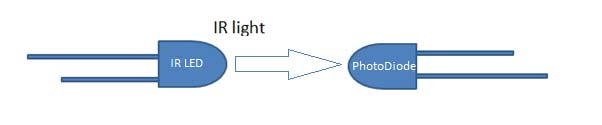
\includegraphics[width=8cm, height=1.6cm]{IR.jpg}
  \caption{IR Principle}
\centering
  \label{fig:IR}
\end{figure}


\subsubsection{PIC Microcontroller}

The system uses PIC16F877A Microcontroller.This powerful (200 nanosecond instruction execution) yet easy-to-program (only 35 single word instructions) CMOS FLASH-based 8-bit microcontroller packs Microchip's powerful PIC® architecture into an 40 package and is upwards compatible with the PIC16C5X, PIC12CXXX and PIC16C7X devices. The PIC16F877A features 256 bytes of EEPROM data memory, self programming, an ICD, 2 Comparators, 8 channels of 10-bit Analog-to-Digital (A/D) converter, 2 capture/compare/PWM functions, the synchronous serial port can be configured as either 3-wire Serial Peripheral Interface (SPI™) or the 2-wire Inter-Integrated Circuit (I²C™) bus and a Universal Asynchronous Receiver Transmitter (USART).
\begin{figure}[H]
  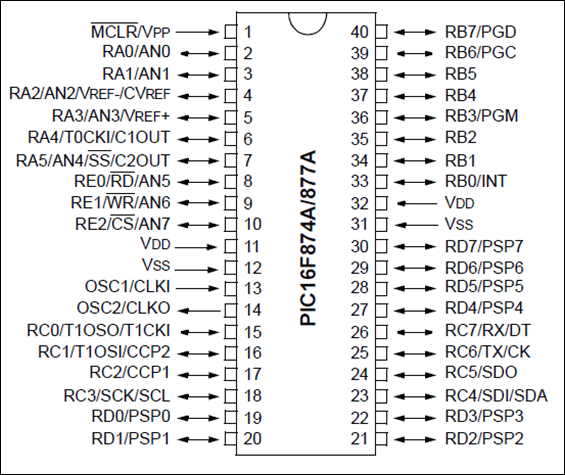
\includegraphics[width=7cm, height=5.2cm]{PIC16F877A-Pinout.png}
  \caption{PIC 16F877A}
\centering
  \label{PIC}
\end{figure}



\subsubsection{LCD Display}

The Model JHD 162A Series LCD is the typical standard HD44780 type of LCD with 16 characters x 2 row LCD module. The LCD displays the state of objects. And indicates ingoing or outgoing direction.

\hfil
\subsubsection{Buzzer}
The Buzzer beeps when an object passes through. Bidrectional objects triggers the buzzer.

\hfil
\subsubsection{Led}
The LED's are used for indicating power status and Bidirectional indication. Red LED is used for outgoing objects. And Green LED is used for incoming objects.

\hfil
\subsubsection{Potentiometer}
The variable resistor or potentiometer is used to adjust the contrast of the LCD

\hfil
\section{Implementation}
The PIC Microcontroller is connected with 20MHz crystal oscillator. The Oscillator requires two 22pF capacitor to stabilize the clock speed. The code is written in Assembly language and uploaded to the PIC Microcontroller’s Flash memory. The Photodiode sensor is connected to the A/D pin of the microcontroller. Microcontroller receives analog value and converts it to digital value and compares it with the threshold value set by user. The microcontroller decides and increase or decreases counter variable and displays it in the LCD display. The counter variable is stored in the EEPROM so that the counter will be safe in case of power loss.
\\
The System is shown below:

\begin{figure}[H]
  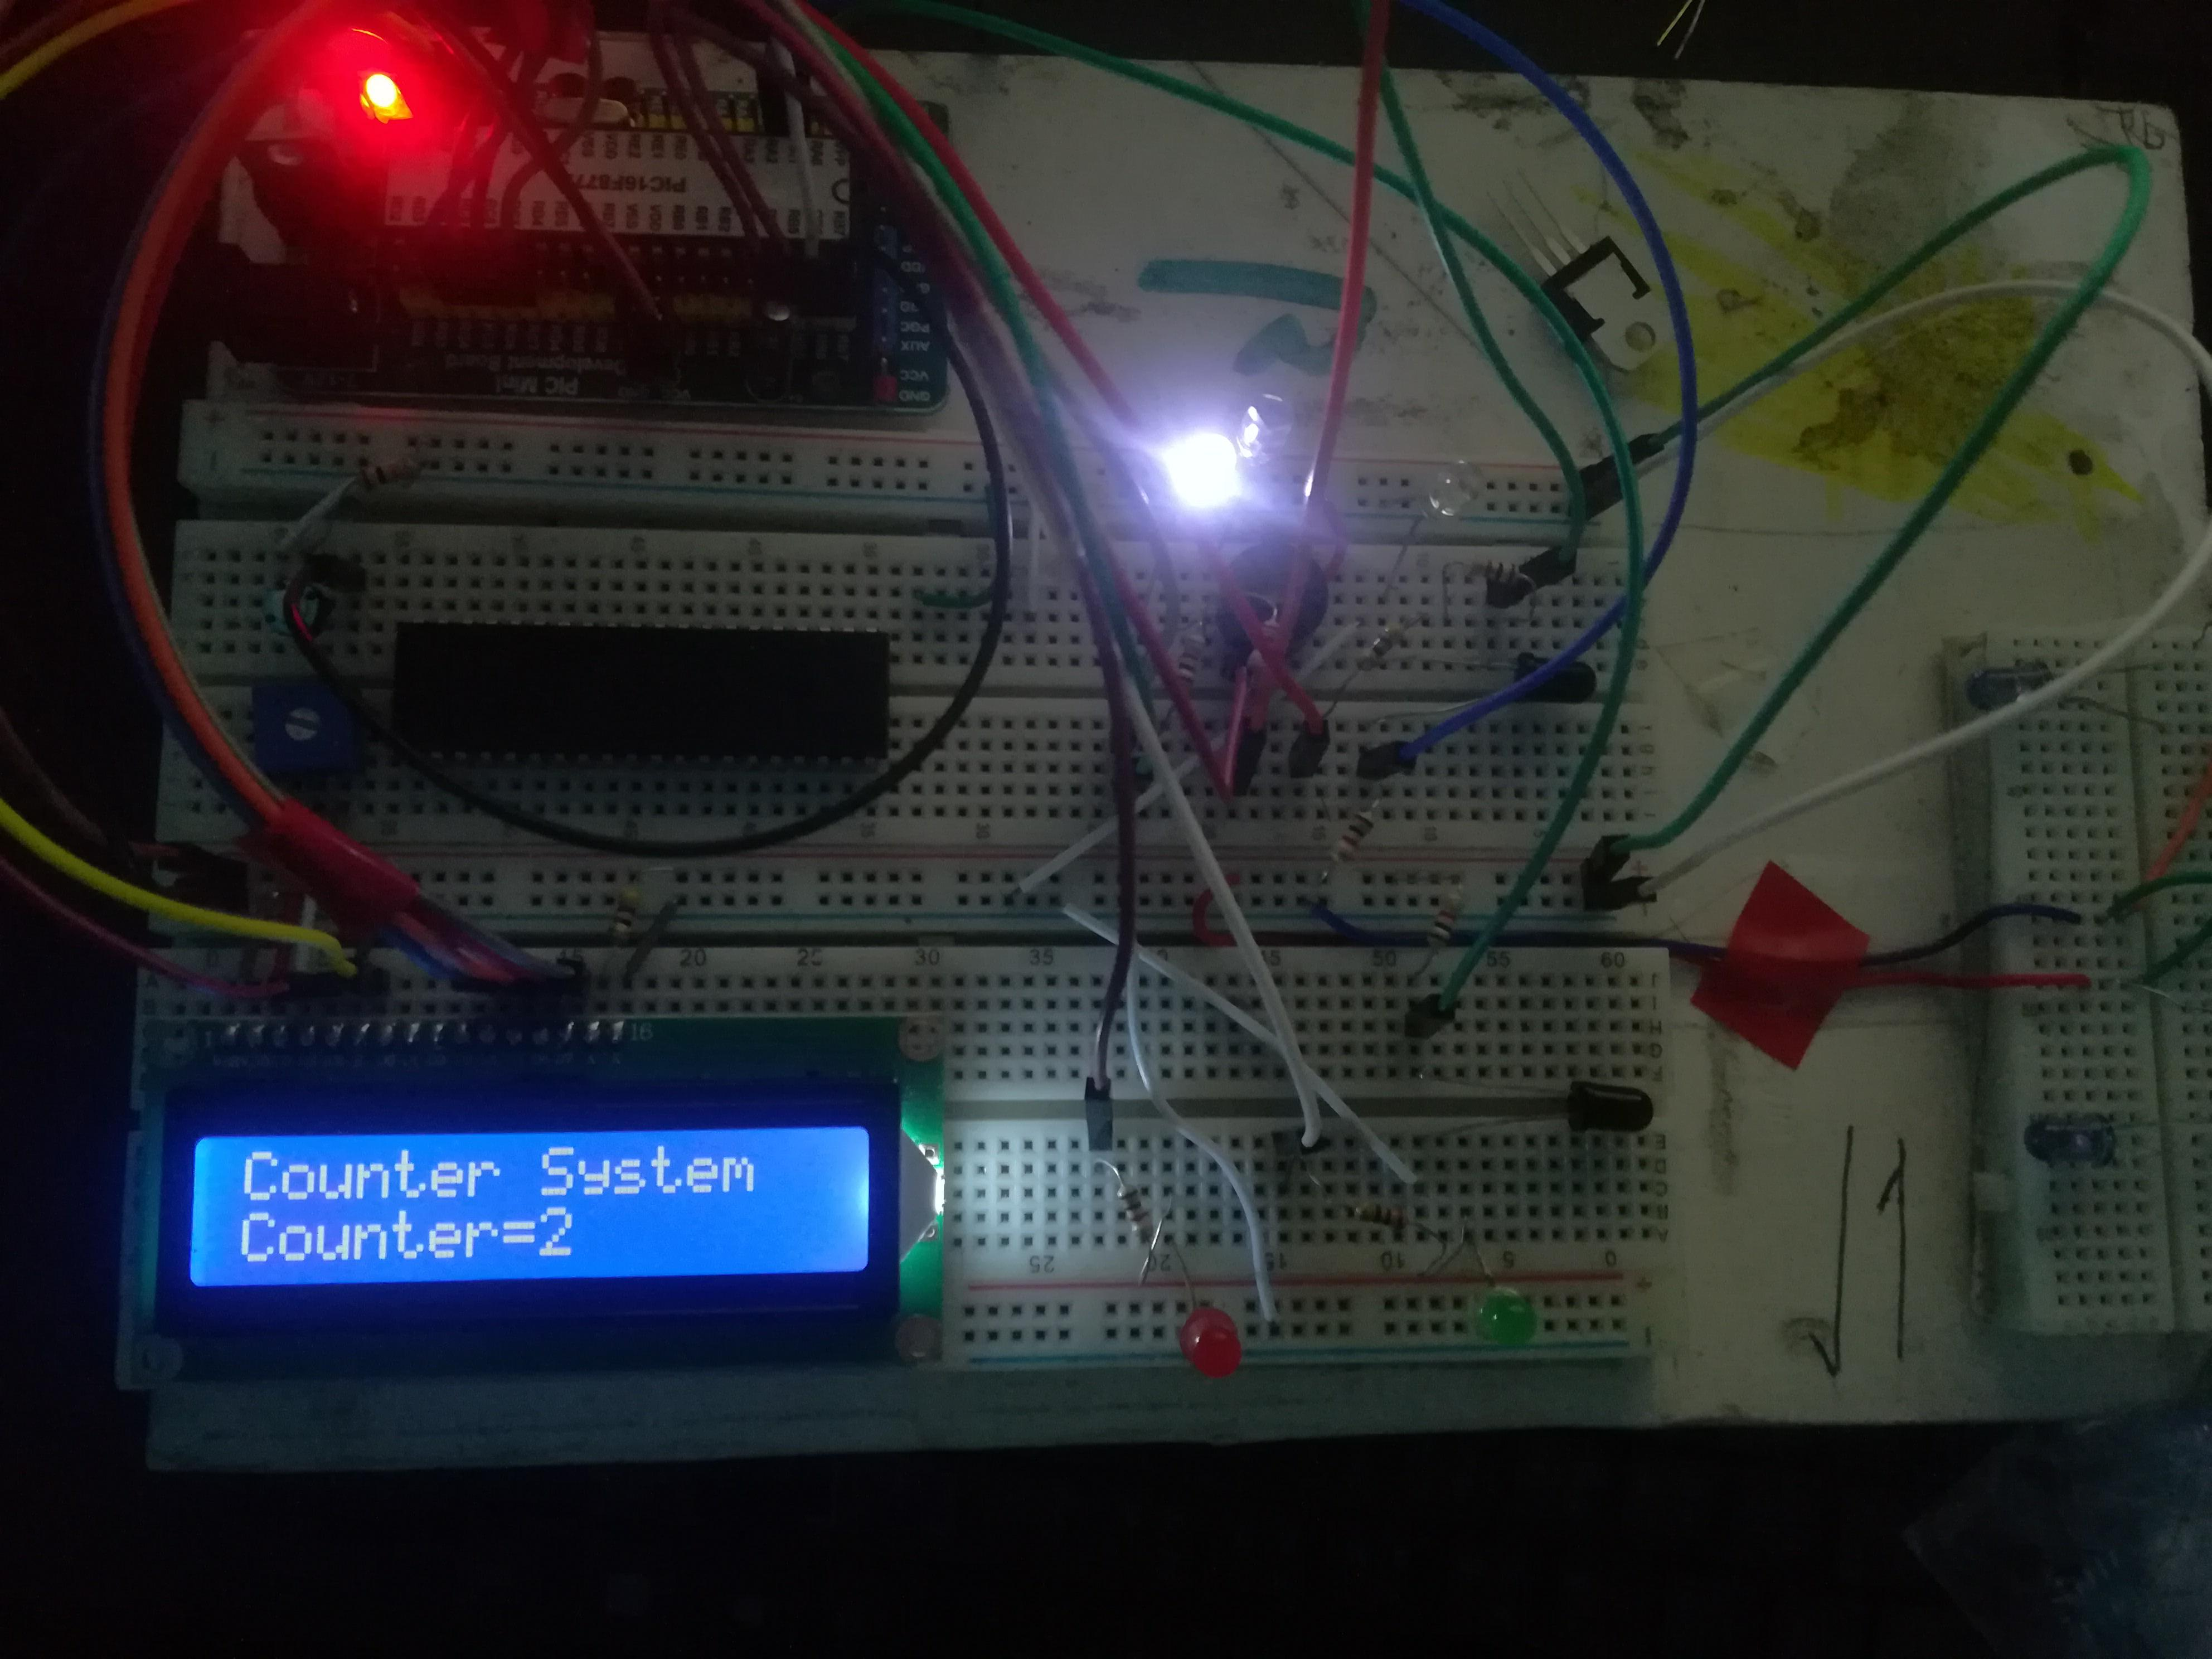
\includegraphics[width=9.1cm, height=7.2cm]{system.jpg}
  \caption{System}
\centering
  \label{fig:system}
\end{figure}
\hfill
\subsection{Circuit And Figures}


The Demo circuit is built in proteus. The proteus Diagram is given below.

\begin{figure}[H]
  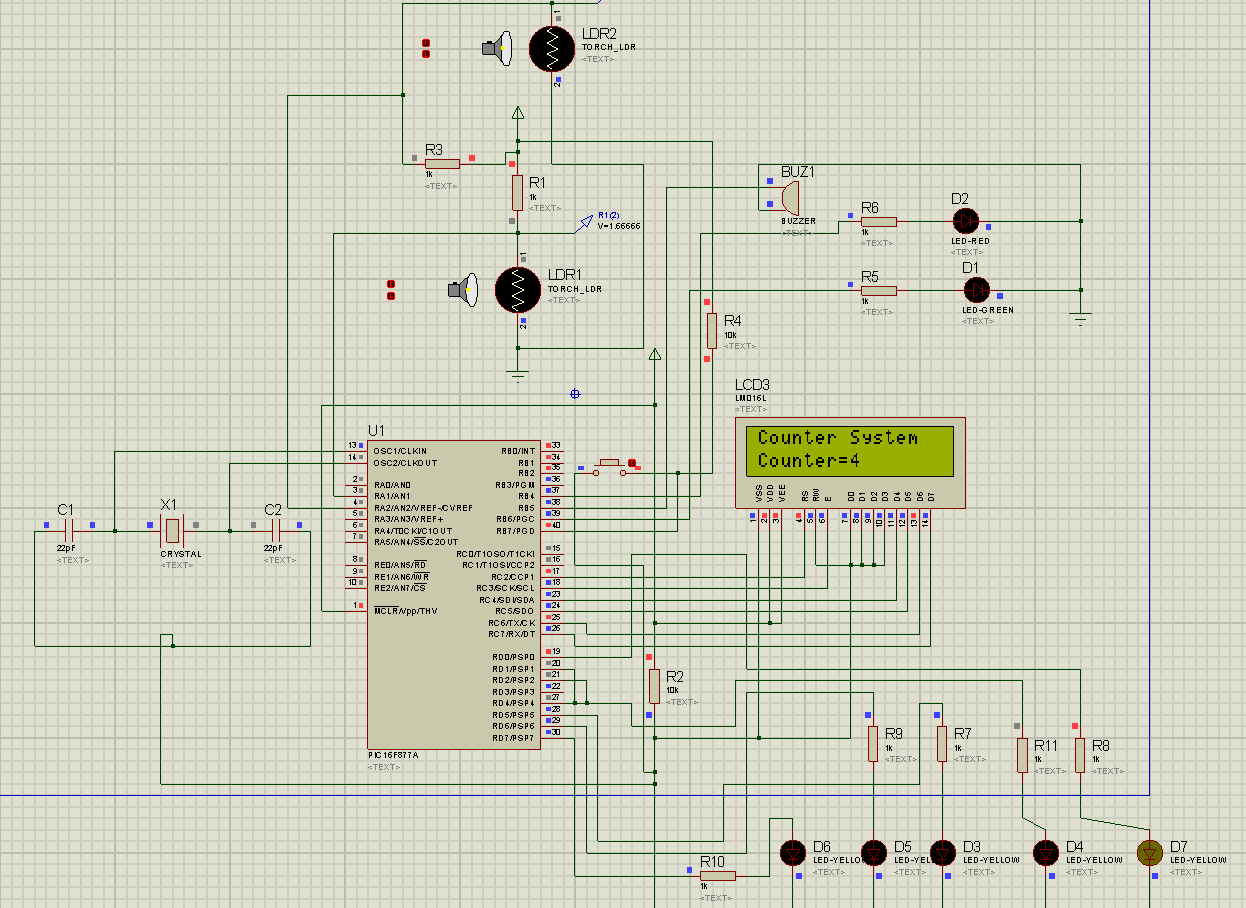
\includegraphics[width=9.7cm, height=8.2cm]{circuit.png}
  \caption{Proteus Circuit}
\centering
  \label{fig:circuit}
\end{figure}





\section{Application}

\subsubsection{}
Indoor Air conditioning can use this system and can adapt to the density of people present and auto adjust power.
\subsubsection{}
Amount of Light and Fan needed to run can be auto adjusted using this circuit.
\subsubsection{}
One example would be the sitting bus service of Dhaka city. They employ a lot of staff members  for counting the passenger. As this counting process becomes annoying passengers also. This simple system could be installed in the door of the buses and the counting process becomes automatic.
\subsubsection{}Factories can install this system and can keep track of their inventory. Product entered and left the facility can be tracked.
\subsubsection{}
 Large scale Auditorium, Movie theatre, Conference halls can install this system and keep count of the people available. Also Mall and Offices can use this system.
 
 
 \section{Limitation}
 This system is low range. Large range implementation of this system will result in error as the IR sensor photodiode gets weak. This limitation can be overcome using Lasers.


% An example of a floating figure using the graphicx package.
% Note that \label must occur AFTER (or within) \caption.
% For figures, \caption should occur after the \includegraphics.
% Note that IEEEtran v1.7 and later has special internal code that
% is designed to preserve the operation of \label within \caption
% even when the captionsoff option is in effect. However, because
% of issues like this, it may be the safest practice to put all your
% \label just after \caption rather than within \caption{}.
%
% Reminder: the "draftcls" or "draftclsnofoot", not "draft", class
% option should be used if it is desired that the figures are to be
% displayed while in draft mode.
%
%\begin{figure}[!t]
%\centering
%\includegraphics[width=2.5in]{myfigure}
% where an .eps filename suffix will be assumed under latex, 
% and a .pdf suffix will be assumed for pdflatex; or what has been declared
% via \DeclareGraphicsExtensions.
%\caption{Simulation results for the network.}
%\label{fig_sim}
%\end{figure}

% Note that the IEEE typically puts floats only at the top, even when this
% results in a large percentage of a column being occupied by floats.


% An example of a double column floating figure using two subfigures.
% (The subfig.sty package must be loaded for this to work.)
% The subfigure \label commands are set within each subfloat command,
% and the \label for the overall figure must come after \caption.
% \hfil is used as a separator to get equal spacing.
% Watch out that the combined width of all the subfigures on a 
% line do not exceed the text width or a line break will occur.
%
%\begin{figure*}[!t]
%\centering
%\subfloat[Case I]{\includegraphics[width=2.5in]{box}%
%\label{fig_first_case}}
%\hfil
%\subfloat[Case II]{\includegraphics[width=2.5in]{box}%
%\label{fig_second_case}}
%\caption{Simulation results for the network.}
%\label{fig_sim}
%\end{figure*}
%
% Note that often IEEE papers with subfigures do not employ subfigure
% captions (using the optional argument to \subfloat[]), but instead will
% reference/describe all of them (a), (b), etc., within the main caption.
% Be aware that for subfig.sty to generate the (a), (b), etc., subfigure
% labels, the optional argument to \subfloat must be present. If a
% subcaption is not desired, just leave its contents blank,
% e.g., \subfloat[].


% An example of a floating table. Note that, for IEEE style tables, the
% \caption command should come BEFORE the table and, given that table
% captions serve much like titles, are usually capitalized except for words
% such as a, an, and, as, at, but, by, for, in, nor, of, on, or, the, to
% and up, which are usually not capitalized unless they are the first or
% last word of the caption. Table text will default to \footnotesize as
% the IEEE normally uses this smaller font for tables.
% The \label must come after \caption as always.
%
%\begin{table}[!t]
%% increase table row spacing, adjust to taste
%\renewcommand{\arraystretch}{1.3}
% if using array.sty, it might be a good idea to tweak the value of
% \extrarowheight as needed to properly center the text within the cells
%\caption{An Example of a Table}
%\label{table_example}
%\centering
%% Some packages, such as MDW tools, offer better commands for making tables
%% than the plain LaTeX2e tabular which is used here.
%\begin{tabular}{|c||c|}
%\hline
%One & Two\\
%\hline
%Three & Four\\
%\hline
%\end{tabular}
%\end{table}


% Note that the IEEE does not put floats in the very first column
% - or typically anywhere on the first page for that matter. Also,
% in-text middle ("here") positioning is typically not used, but it
% is allowed and encouraged for Computer Society conferences (but
% not Computer Society journals). Most IEEE journals/conferences use
% top floats exclusively. 
% Note that, LaTeX2e, unlike IEEE journals/conferences, places
% footnotes above bottom floats. This can be corrected via the
% \fnbelowfloat command of the stfloats package.


\section{Conclusion}

The system is overall simplified counting solution for most use cases. This system can ultimately help reduce the overall cost of any counting mechanism service and be easy to adapt. The system saves data in EEPROM and thus avoid the loss of data due to power loss.The system has scope for introducing new functionality and can be easily upgraded. A Lot of small companies and business can greatly benefit themselves by installing this system.



\vspace{50mm} %5mm vertical space
\section{Code:}
Assembly Code of the System :
\begin{lstlisting}

ORG	0x0000	; 

; _LightSet:
; 
;         MOVLW      128
;         MOVWF      R0+0
;         MOVLW      128
;         XORWF      FARG_LightSet_countD+1, 0
;         SUBWF      R0+0, 0
;         BTFSS      STATUS+0, 2
;         GOTO       L__LightSet45
;         MOVF       FARG_LightSet_countD+0, 0
;         SUBLW      0
; L__LightSet45:
;         BTFSS      STATUS+0, 0
;         GOTO       L_LightSet0
;         CLRF       PORTD+0
;         GOTO       L_LightSet1
; L_LightSet0:
;         MOVLW      128
;         MOVWF      R0+0
;         MOVLW      128
;         XORWF      FARG_LightSet_countD+1, 0
;         SUBWF      R0+0, 0
;         BTFSS      STATUS+0, 2
;         GOTO       L__LightSet46
;         MOVF       FARG_LightSet_countD+0, 0
;         SUBLW      0
; L__LightSet46:
;         BTFSC      STATUS+0, 0
;         GOTO       L_LightSet4
;         MOVLW      128
;         XORWF      FARG_LightSet_countD+1, 0
;         MOVWF      R0+0
;         MOVLW      128
;         SUBWF      R0+0, 0
;         BTFSS      STATUS+0, 2
;         GOTO       L__LightSet47
;         MOVLW      3
;         SUBWF      FARG_LightSet_countD+0, 0
; L__LightSet47:
;         BTFSC      STATUS+0, 0
;         GOTO       L_LightSet4
; L__LightSet43:
;         MOVLW      1
;         MOVWF      PORTD+0
;         GOTO       L_LightSet5
; L_LightSet4:
;         MOVLW      128
;         XORWF      FARG_LightSet_countD+1, 0
;         MOVWF      R0+0
;         MOVLW      128
;         SUBWF      R0+0, 0
;         BTFSS      STATUS+0, 2
;         GOTO       L__LightSet48
;         MOVLW      3
;         SUBWF      FARG_LightSet_countD+0, 0
; L__LightSet48:
;         BTFSS      STATUS+0, 0
;         GOTO       L_LightSet8
;         MOVLW      128
;         XORWF      FARG_LightSet_countD+1, 0
;         MOVWF      R0+0
;         MOVLW      128
;         SUBWF      R0+0, 0
;         BTFSS      STATUS+0, 2
;         GOTO       L__LightSet49
;         MOVLW      5
;         SUBWF      FARG_LightSet_countD+0, 0
; L__LightSet49:
;         BTFSC      STATUS+0, 0
;         GOTO       L_LightSet8
; L__LightSet42:
;         MOVLW      7
;         MOVWF      PORTD+0
;         GOTO       L_LightSet9
; L_LightSet8:
;         MOVLW      128
;         XORWF      FARG_LightSet_countD+1, 0
;         MOVWF      R0+0
;         MOVLW      128
;         SUBWF      R0+0, 0
;         BTFSS      STATUS+0, 2
;         GOTO       L__LightSet50
;         MOVLW      5
;         SUBWF      FARG_LightSet_countD+0, 0
; L__LightSet50:
;         BTFSS      STATUS+0, 0
;         GOTO       L_LightSet12
;         MOVLW      128
;         XORWF      FARG_LightSet_countD+1, 0
;         MOVWF      R0+0
;         MOVLW      128
;         SUBWF      R0+0, 0
;         BTFSS      STATUS+0, 2
;         GOTO       L__LightSet51
;         MOVLW      10
;         SUBWF      FARG_LightSet_countD+0, 0
; L__LightSet51:
;         BTFSC      STATUS+0, 0
;         GOTO       L_LightSet12
; L__LightSet41:
;         MOVLW      63
;         MOVWF      PORTD+0
;         GOTO       L_LightSet13
; L_LightSet12:
;         MOVLW      255
;         MOVWF      PORTD+0
; L_LightSet13:
; L_LightSet9:
; L_LightSet5:
; L_LightSet1:
; L_end_LightSet:
;         RETURN
; 
; _main:
; 
;         MOVLW      128
;         MOVWF      ADCON1+0
;         MOVLW      255
;         MOVWF      TRISA+0
;         MOVLW      63
;         MOVWF      TRISC+0
;         MOVLW      128
;         MOVWF      TRISB+0
;         BSF        TRISB+0, 7
;         CLRF       TRISD+0
;         CLRF       PORTD+0
;         MOVLW      2
;         MOVWF      FARG_EEPROM_Write_Address+0
;         MOVLW      5
;         MOVWF      FARG_EEPROM_Write_data_+0
;         CALL       _EEPROM_Write+0
;         MOVLW      3
;         MOVWF      R11+0
;         MOVLW      138
;         MOVWF      R12+0
;         MOVLW      85
;         MOVWF      R13+0
; L_main14:
;         DECFSZ     R13+0, 1
;         GOTO       L_main14
;         DECFSZ     R12+0, 1
;         GOTO       L_main14
;         DECFSZ     R11+0, 1
;         GOTO       L_main14
;         NOP
;         NOP
;         MOVLW      2
;         MOVWF      FARG_EEPROM_Read_Address+0
;         CALL       _EEPROM_Read+0
;         MOVF       R0+0, 0
;         MOVWF      _count+0
;         CALL       _Lcd_Init+0
;         MOVLW      1
;         MOVWF      FARG_Lcd_Cmd_out_char+0
;         CALL       _Lcd_Cmd+0
;         MOVLW      12
;         MOVWF      FARG_Lcd_Cmd_out_char+0
;         CALL       _Lcd_Cmd+0
;         MOVLW      17
;         MOVWF      FARG_EEPROM_Read_Address+0
;         CALL       _EEPROM_Read+0
;         MOVF       R0+0, 0
;         MOVWF      _read+0
;         MOVF       R0+0, 0
;         SUBLW      0
;         BTFSC      STATUS+0, 0
;         GOTO       L_main15
;         MOVF       _read+0, 0
;         MOVWF      _count+0
;         MOVF       _read+0, 0
;         MOVWF      _countD+0
;         CLRF       _countD+1
;         GOTO       L_main16
; L_main15:
;         CLRF       _count+0
;         CLRF       PORTD+0
;         CLRF       _countD+0
;         CLRF       _countD+1
; L_main16:
; L_main17:
;         MOVLW      1
;         MOVWF      FARG_ADC_Read_channel+0
;         CALL       _ADC_Read+0
;         MOVF       R0+0, 0
;         MOVWF      _adc+0
;         MOVF       R0+1, 0
;         MOVWF      _adc+1
;         MOVLW      2
;         MOVWF      FARG_ADC_Read_channel+0
;         CALL       _ADC_Read+0
;         MOVF       R0+0, 0
;         MOVWF      _adc2+0
;         MOVF       R0+1, 0
;         MOVWF      _adc2+1
;         MOVF       _adc+1, 0
;         SUBLW      1
;         BTFSS      STATUS+0, 2
;         GOTO       L__main53
;         MOVF       _adc+0, 0
;         SUBLW      144
; L__main53:
;         BTFSC      STATUS+0, 0
;         GOTO       L_main20
;         INCF       _count+0, 1
;         MOVLW      1
;         MOVWF      FARG_Lcd_Cmd_out_char+0
;         CALL       _Lcd_Cmd+0
;         MOVLW      1
;         MOVWF      FARG_Lcd_Out_row+0
;         MOVLW      1
;         MOVWF      FARG_Lcd_Out_column+0
;         MOVLW      ?lstr1_MyProject+0
;         MOVWF      FARG_Lcd_Out_text+0
;         CALL       _Lcd_Out+0
;         MOVLW      32
;         MOVWF      PORTB+0
;         MOVLW      2
;         MOVWF      R11+0
;         MOVLW      69
;         MOVWF      R12+0
;         MOVLW      169
;         MOVWF      R13+0
; L_main21:
;         DECFSZ     R13+0, 1
;         GOTO       L_main21
;         DECFSZ     R12+0, 1
;         GOTO       L_main21
;         DECFSZ     R11+0, 1
;         GOTO       L_main21
;         NOP
;         NOP
;         MOVLW      64
;         MOVWF      PORTB+0
;         INCF       _countD+0, 1
;         BTFSC      STATUS+0, 2
;         INCF       _countD+1, 1
;         CLRF       _i+0
; L_main22:
;         MOVLW      4
;         SUBWF      _i+0, 0
;         BTFSC      STATUS+0, 0
;         GOTO       L_main23
;         MOVLW      28
;         MOVWF      FARG_Lcd_Cmd_out_char+0
;         CALL       _Lcd_Cmd+0
;         MOVLW      13
;         MOVWF      R11+0
;         MOVLW      175
;         MOVWF      R12+0
;         MOVLW      182
;         MOVWF      R13+0
; L_main25:
;         DECFSZ     R13+0, 1
;         GOTO       L_main25
;         DECFSZ     R12+0, 1
;         GOTO       L_main25
;         DECFSZ     R11+0, 1
;         GOTO       L_main25
;         NOP
;         INCF       _i+0, 1
;         GOTO       L_main22
; L_main23:
;         MOVLW      1
;         MOVWF      FARG_Lcd_Cmd_out_char+0
;         CALL       _Lcd_Cmd+0
;         CLRF       PORTB+0
;         MOVF       _countD+0, 0
;         MOVWF      FARG_LightSet_countD+0
;         MOVF       _countD+1, 0
;         MOVWF      FARG_LightSet_countD+1
;         CALL       _LightSet+0
;         GOTO       L_main26
; L_main20:
;         MOVF       _adc2+1, 0
;         SUBLW      1
;         BTFSS      STATUS+0, 2
;         GOTO       L__main54
;         MOVF       _adc2+0, 0
;         SUBLW      144
; L__main54:
;         BTFSC      STATUS+0, 0
;         GOTO       L_main27
;         MOVF       _count+0, 0
;         SUBLW      0
;         BTFSS      STATUS+0, 0
;         GOTO       L_main28
;         CLRF       _count+0
;         MOVLW      21
;         MOVWF      R11+0
;         MOVLW      75
;         MOVWF      R12+0
;         MOVLW      190
;         MOVWF      R13+0
; L_main29:
;         DECFSZ     R13+0, 1
;         GOTO       L_main29
;         DECFSZ     R12+0, 1
;         GOTO       L_main29
;         DECFSZ     R11+0, 1
;         GOTO       L_main29
;         NOP
;         CLRF       PORTD+0
;         CLRF       _countD+0
;         CLRF       _countD+1
;         CLRF       FARG_LightSet_countD+0
;         CLRF       FARG_LightSet_countD+1
;         CALL       _LightSet+0
;         GOTO       L_main30
; L_main28:
;         MOVLW      32
;         MOVWF      PORTB+0
;         MOVLW      2
;         MOVWF      R11+0
;         MOVLW      69
;         MOVWF      R12+0
;         MOVLW      169
;         MOVWF      R13+0
; L_main31:
;         DECFSZ     R13+0, 1
;         GOTO       L_main31
;         DECFSZ     R12+0, 1
;         GOTO       L_main31
;         DECFSZ     R11+0, 1
;         GOTO       L_main31
;         NOP
;         NOP
;         MOVLW      16
;         MOVWF      PORTB+0
;         DECF       _count+0, 1
;         MOVLW      1
;         SUBWF      _countD+0, 1
;         BTFSS      STATUS+0, 0
;         DECF       _countD+1, 1
;         MOVLW      1
;         MOVWF      FARG_Lcd_Cmd_out_char+0
;         CALL       _Lcd_Cmd+0
;         MOVLW      1
;         MOVWF      FARG_Lcd_Out_row+0
;         MOVLW      1
;         MOVWF      FARG_Lcd_Out_column+0
;         MOVLW      ?lstr2_MyProject+0
;         MOVWF      FARG_Lcd_Out_text+0
;         CALL       _Lcd_Out+0
;         CLRF       _i+0
; L_main32:
;         MOVLW      4
;         SUBWF      _i+0, 0
;         BTFSC      STATUS+0, 0
;         GOTO       L_main33
;         MOVLW      28
;         MOVWF      FARG_Lcd_Cmd_out_char+0
;         CALL       _Lcd_Cmd+0
;         MOVLW      13
;         MOVWF      R11+0
;         MOVLW      175
;         MOVWF      R12+0
;         MOVLW      182
;         MOVWF      R13+0
; L_main35:
;         DECFSZ     R13+0, 1
;         GOTO       L_main35
;         DECFSZ     R12+0, 1
;         GOTO       L_main35
;         DECFSZ     R11+0, 1
;         GOTO       L_main35
;         NOP
;         INCF       _i+0, 1
;         GOTO       L_main32
; L_main33:
; L_main30:
;         MOVLW      1
;         MOVWF      FARG_Lcd_Cmd_out_char+0
;         CALL       _Lcd_Cmd+0
;         CLRF       PORTB+0
;         MOVF       _countD+0, 0
;         MOVWF      FARG_LightSet_countD+0
;         MOVF       _countD+1, 0
;         MOVWF      FARG_LightSet_countD+1
;         CALL       _LightSet+0
; L_main27:
; L_main26:
;         MOVF       _countD+0, 0
;         MOVWF      FARG_LightSet_countD+0
;         MOVF       _countD+1, 0
;         MOVWF      FARG_LightSet_countD+1
;         CALL       _LightSet+0
;         MOVLW      1
;         MOVWF      FARG_Lcd_Out_row+0
;         MOVLW      1
;         MOVWF      FARG_Lcd_Out_column+0
;         MOVLW      ?lstr3_MyProject+0
;         MOVWF      FARG_Lcd_Out_text+0
;         CALL       _Lcd_Out+0
;         MOVLW      2
;         MOVWF      FARG_Lcd_Out_row+0
;         MOVLW      1
;         MOVWF      FARG_Lcd_Out_column+0
;         MOVLW      ?lstr4_MyProject+0
;         MOVWF      FARG_Lcd_Out_text+0
;         CALL       _Lcd_Out+0
;         MOVF       _count+0, 0
;         MOVWF      FARG_ShortToStr_input+0
;         MOVLW      _counterArray+0
;         MOVWF      FARG_ShortToStr_output+0
;         CALL       _ShortToStr+0
;         MOVLW      _counterArray+0
;         MOVWF      FARG_Ltrim_string+0
;         CALL       _Ltrim+0
;         MOVF       R0+0, 0
;         MOVWF      _t+0
;         MOVLW      2
;         MOVWF      FARG_Lcd_Out_row+0
;         MOVLW      9
;         MOVWF      FARG_Lcd_Out_column+0
;         MOVF       R0+0, 0
;         MOVWF      FARG_Lcd_Out_text+0
;         CALL       _Lcd_Out+0
;         BTFSC      PORTB+0, 7
;         GOTO       L_main36
;         MOVLW      3
;         MOVWF      R11+0
;         MOVLW      138
;         MOVWF      R12+0
;         MOVLW      85
;         MOVWF      R13+0
; L_main37:
;         DECFSZ     R13+0, 1
;         GOTO       L_main37
;         DECFSZ     R12+0, 1
;         GOTO       L_main37
;         DECFSZ     R11+0, 1
;         GOTO       L_main37
;         NOP
;         NOP
;         BTFSC      PORTB+0, 7
;         GOTO       L_main38
;         MOVLW      1
;         MOVWF      FARG_Lcd_Cmd_out_char+0
;         CALL       _Lcd_Cmd+0
;         MOVLW      3
;         MOVWF      R11+0
;         MOVLW      138
;         MOVWF      R12+0
;         MOVLW      85
;         MOVWF      R13+0
; L_main39:
;         DECFSZ     R13+0, 1
;         GOTO       L_main39
;         DECFSZ     R12+0, 1
;         GOTO       L_main39
;         DECFSZ     R11+0, 1
;         GOTO       L_main39
;         NOP
;         NOP
;         MOVLW      1
;         MOVWF      FARG_Lcd_Out_row+0
;         MOVLW      1
;         MOVWF      FARG_Lcd_Out_column+0
;         MOVLW      ?lstr5_MyProject+0
;         MOVWF      FARG_Lcd_Out_text+0
;         CALL       _Lcd_Out+0
;         CLRF       _count+0
;         CLRF       _countD+0
;         CLRF       _countD+1
; L_main38:
; L_main36:
;         MOVLW      6
;         MOVWF      R11+0
;         MOVLW      19
;         MOVWF      R12+0
;         MOVLW      173
;         MOVWF      R13+0
; L_main40:
;         DECFSZ     R13+0, 1
;         GOTO       L_main40
;         DECFSZ     R12+0, 1
;         GOTO       L_main40
;         DECFSZ     R11+0, 1
;         GOTO       L_main40
;         NOP
;         NOP
;         MOVLW      17
;         MOVWF      FARG_EEPROM_Write_Address+0
;         MOVF       _count+0, 0
;         MOVWF      FARG_EEPROM_Write_data_+0
;         CALL       _EEPROM_Write+0
;         GOTO       L_main17
; L_end_main:
;         GOTO       $+0

		END
\end{lstlisting}



% conference papers do not normally have an appendix


% use section* for acknowledgment


\section*{Acknowledgment}


The author would like to thank microchip for PIC tutorials.






% trigger a \newpage just before the given reference
% number - used to balance the columns on the last page
% adjust value as needed - may need to be readjusted if
% the document is modified later
%\IEEEtriggeratref{8}
% The "triggered" command can be changed if desired:
%\IEEEtriggercmd{\enlargethispage{-5in}}

% references section

% can use a bibliography generated by BibTeX as a .bbl file
% BibTeX documentation can be easily obtained at:
% http://mirror.ctan.org/biblio/bibtex/contrib/doc/
% The IEEEtran BibTeX style support page is at:
% http://www.michaelshell.org/tex/ieeetran/bibtex/
%\bibliographystyle{IEEEtran}
% argument is your BibTeX string definitions and bibliography database(s)
%\bibliography{IEEEabrv,../bib/paper}
%
% <OR> manually copy in the resultant .bbl file
% set second argument of \begin to the number of references
% (used to reserve space for the reference number labels box)
\begin{thebibliography}{1}

\bibitem{IEEEhowto:kopka}
Microchip Forum for PIC .
\bibitem{IEEEhowto:kopka}
Getting started with PIC Microcontroller Tutorial\\
\url{https://circuitdigest.com/microcontroller-projects/getting-started-with-pic-microcontroller}\end{thebibliography}




% that's all folks

\end{document}


